

\lstset{
    breaklines=true,
    postbreak=\mbox{\textcolor{red}{$\hookrightarrow$}\space},
    frame=single,
    numbers=left,
    numberstyle=\tiny\color{gray},
    basicstyle=\ttfamily\footnotesize,
    keywordstyle=\color{blue},
    commentstyle=\color{green!40!black},
    stringstyle=\color{orange},
    showstringspaces=false,
    columns=flexible,
    keepspaces=true,
    breakatwhitespace=false
}

\lstdefinestyle{bashstyle}{
  language=bash,
  basicstyle=\ttfamily\footnotesize,
  breaklines=true,
  postbreak=\mbox{\textcolor{red}{$\hookrightarrow$}\space},
  commentstyle=\color{green!40!black},
  keywordstyle=\color{blue},
  stringstyle=\color{orange},
  numbers=left,
  numberstyle=\tiny\color{gray},
  stepnumber=1,
  numbersep=5pt,
  backgroundcolor=\color{white},
  showspaces=false,
  showstringspaces=false,
  showtabs=false,
  tabsize=2,
  captionpos=b,
  breakatwhitespace=false,
  breakautoindent=true,
  escapeinside={\%*}{*)},
  linewidth=\textwidth,
  basewidth=0.5em,
}
\lstset{style=bashstyle}


\tableofcontents
Definizione Vulnerabilità


\begin{center}
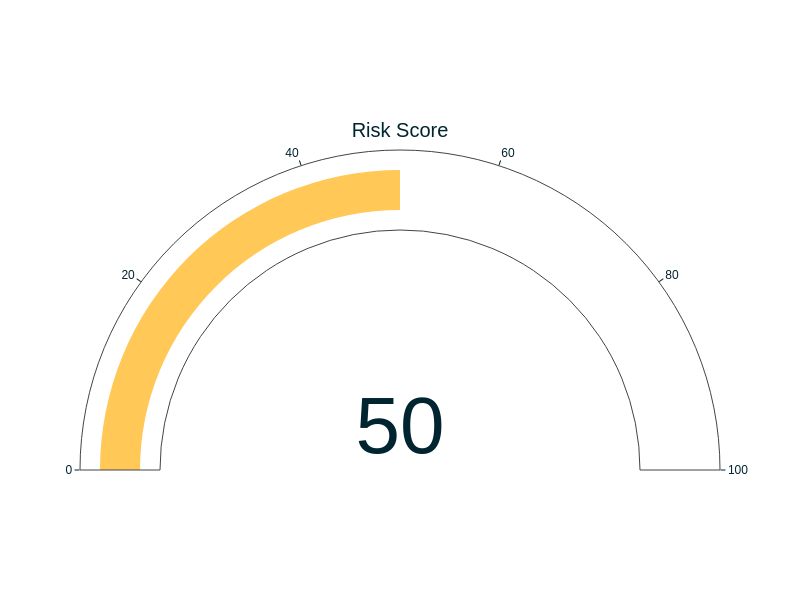
\includegraphics[width=\linewidth]{pngs/0_1.png}
\vspace{1cm}\caption{First image of Chapter 1}
\end{center}

\section{Gravità Critica}
\begin{itemize}
\item Lo sfruttamento è semplice e di solito comporta una compromissione a livello di sistema. Si consiglia di pianificare un'azione correttiva e applicare una patch immediatamente.
\end{itemize}
\section{Gravità Alta}
\begin{itemize}
\item Lo sfruttamento è più difficile, ma potrebbe causare l'elevazione dei privilegi e potenzialmente la perdita di dati o interruzioni del servizio. Si consiglia di pianificare un'azione correttiva e applicare una patch il prima possibile.
\end{itemize}
\section{Gravità Media}
\begin{itemize}
\item Le vulnerabilità esistono, ma richiedono passaggi aggiuntivi, come l'ingegneria sociale. Si consiglia di pianificare un'azione correttiva e applicare una patch dopo che le problematiche ad alta priorità sono state risolte.
\end{itemize}
\section{Gravità Bassa}
\begin{itemize}
\item Le vulnerabilità non sono sfruttabili, ma aumentano la superficie d'attacco di un'organizzazione. Si consiglia di pianificare un'azione correttiva e applicare una patch durante la prossima finestra di manutenzione.
\end{itemize}
\section{Gravità Informativa}
\begin{itemize}
\item Non esiste alcuna vulnerabilità nota. Vengono fornite informazioni aggiuntive riguardanti elementi osservati durante i test, controlli solidi e documentazione aggiuntiva.
\end{itemize}

\chapter{Analisi della Panoramica di Sicurezza}

\section{Panoramica della Postura di Sicurezza e Livello di Rischio Complessivo}

La panoramica di sicurezza presentata evidenzia un numero significativo di vulnerabilità, con un totale di 174 vulnerabilità identificate. Il punteggio di rischio complessivo è stato calcolato su 55/100, il che indica un livello di rischio medio. Nonostante ciò, la mancanza di vulnerabilità critiche e alte è rassicurante, poiché queste rappresentano il tipo di vulnerabilità più pericoloso per l'organizzazione.

\section{Considerazioni sul Numero Totale di Vulnerabilità}

Il numero totale di vulnerabilità identificate (174) è significativo e suggerisce che l'organizzazione potrebbe avere una superficie d'attacco più ampia di quanto desiderato. Questo può essere dovuto a vari fattori, come l'età del sistema, la complessità dell'infrastruttura IT e la mancanza di un'adeguata gestione della sicurezza. È importante identificare e correggere queste vulnerabilità per ridurre il rischio di attacchi e garantire la protezione dei dati sensibili.

\section{Suddivisione dei Tipi di Vulnerabilità}

La panoramica di sicurezza evidenzia una suddivisione dei tipi di vulnerabilità come segue:
\begin{itemize}
\item \textbf{Vulnerabilità Critiche (0)}: Non sono presenti vulnerabilità critiche, il che significa che non esistono vulnerabilità che possano essere facilmente sfruttate per compromettere la sicurezza dell'organizzazione.
\item \textbf{Vulnerabilità Alte (0)}: Non sono presenti vulnerabilità alte, il che significa che non esistono vulnerabilità che possano essere facilmente sfruttate per compromettere la sicurezza dell'organizzazione.
\item \textbf{Vulnerabilità Medie (4)}: Sono presenti 4 vulnerabilità medie, il che significa che queste richiedono passaggi aggiuntivi, come l'ingegneria sociale, per essere sfruttate. È importante pianificare un'azione correttiva e applicare una patch per correggere queste vulnerabilità.
\item \textbf{Vulnerabilità Basse (0)}: Non sono presenti vulnerabilità basse, il che significa che non esistono vulnerabilità che non possano essere sfruttate per compromettere la sicurezza dell'organizzazione.
\end{itemize}
In sintesi, la panoramica di sicurezza evidenzia un numero significativo di vulnerabilità, ma la mancanza di vulnerabilità critiche e alte è rassicurante. È importante identificare e correggere le vulnerabilità medie per ridurre il rischio di attacchi e garantire la protezione dei dati sensibili.


\begin{center}
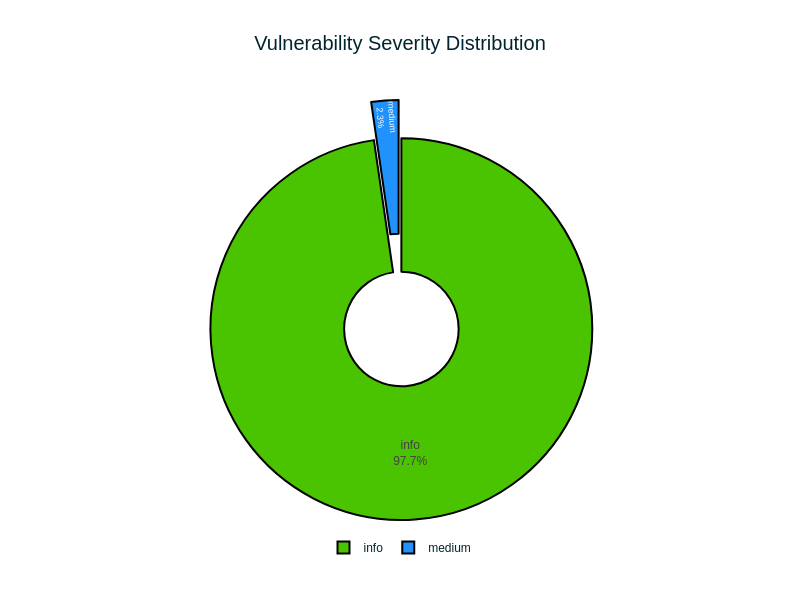
\includegraphics[width=\linewidth]{pngs/1_1.png}
\vspace{1cm}\caption{Images related to Chapter 2}
\end{center}
\chapter{Analisi della Distribuzione delle Gravità delle Vulnerabilità}

\section{Riepilogo della Distribuzione delle Gravità}

La distribuzione delle gravità delle vulnerabilità è la seguente:
\begin{itemize}
\item \textbf{Gravità Critica (High)}: 170
\item \textbf{Gravità Media (Medium)}: 4
\end{itemize}
\section{Livello di Gravità più Comune}

Il livello di gravità più comune è la \textbf{Gravità Critica (High)}, con 170 vulnerabilità.

\section{Percentuale di ciascun livello di Gravità}
\begin{itemize}
\item \textbf{Gravità Critica (High)}: 170 / (170 + 4) = 97,4\%
\item \textbf{Gravità Media (Medium)}: 4 / (170 + 4) = 2,6\%
\end{itemize}
\section{Impatto delle Vulnerabilità Critiche e Alte}

Le vulnerabilità critiche e alte possono causare una compromissione a livello di sistema e potenzialmente la perdita di dati o interruzioni del servizio. È fondamentale pianificare un'azione correttiva e applicare una patch immediatamente per mitigare questi rischi.

\section{Urgenza della Risoluzione}

È essenziale risolvere queste vulnerabilità critiche e alte il prima possibile per garantire la sicurezza e la conformità della sistema.

\section{Rischio cumulativo delle Vulnerabilità Medie e Basse}

Le vulnerabilità medie e basse non sono direttamente correlate a una compromissione a livello di sistema, ma possono aumentare la superficie d'attacco di un'organizzazione. Tuttavia, il rischio cumulativo di queste vulnerabilità è limitato e non rappresenta un rischio significativo per la sicurezza del sistema.

\section{Rischio complessivo e Impatto su Conformità/Sicurezza}

Il rischio complessivo è determinato principalmente dalle vulnerabilità critiche e alte, che rappresentano un rischio significativo per la sicurezza del sistema. Tuttavia, la distribuzione delle gravità è relativamente bassa, il che significa che il rischio complessivo è limitato. È fondamentale concentrarsi sulla risoluzione delle vulnerabilità critiche e alte e pianificare un'azione correttiva per mitigare i rischi.


\begin{center}
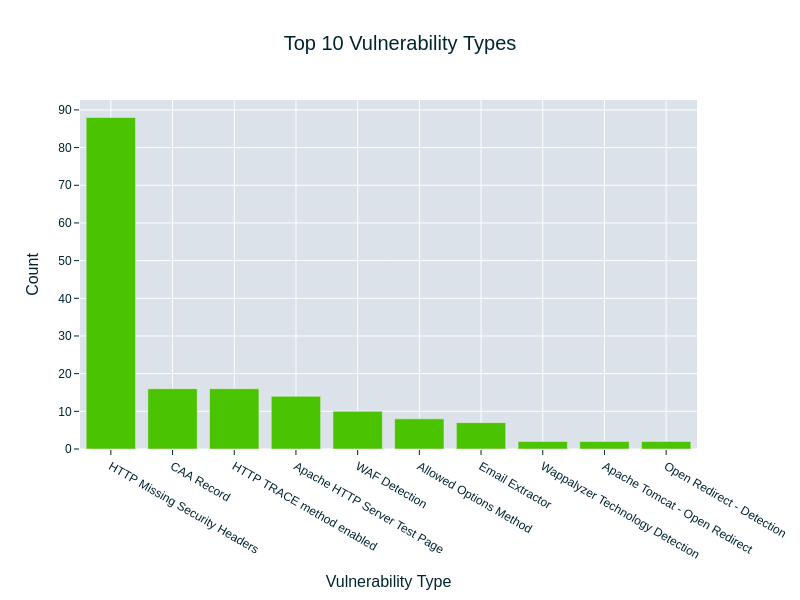
\includegraphics[width=\linewidth]{pngs/2_1.png}
\vspace{1cm}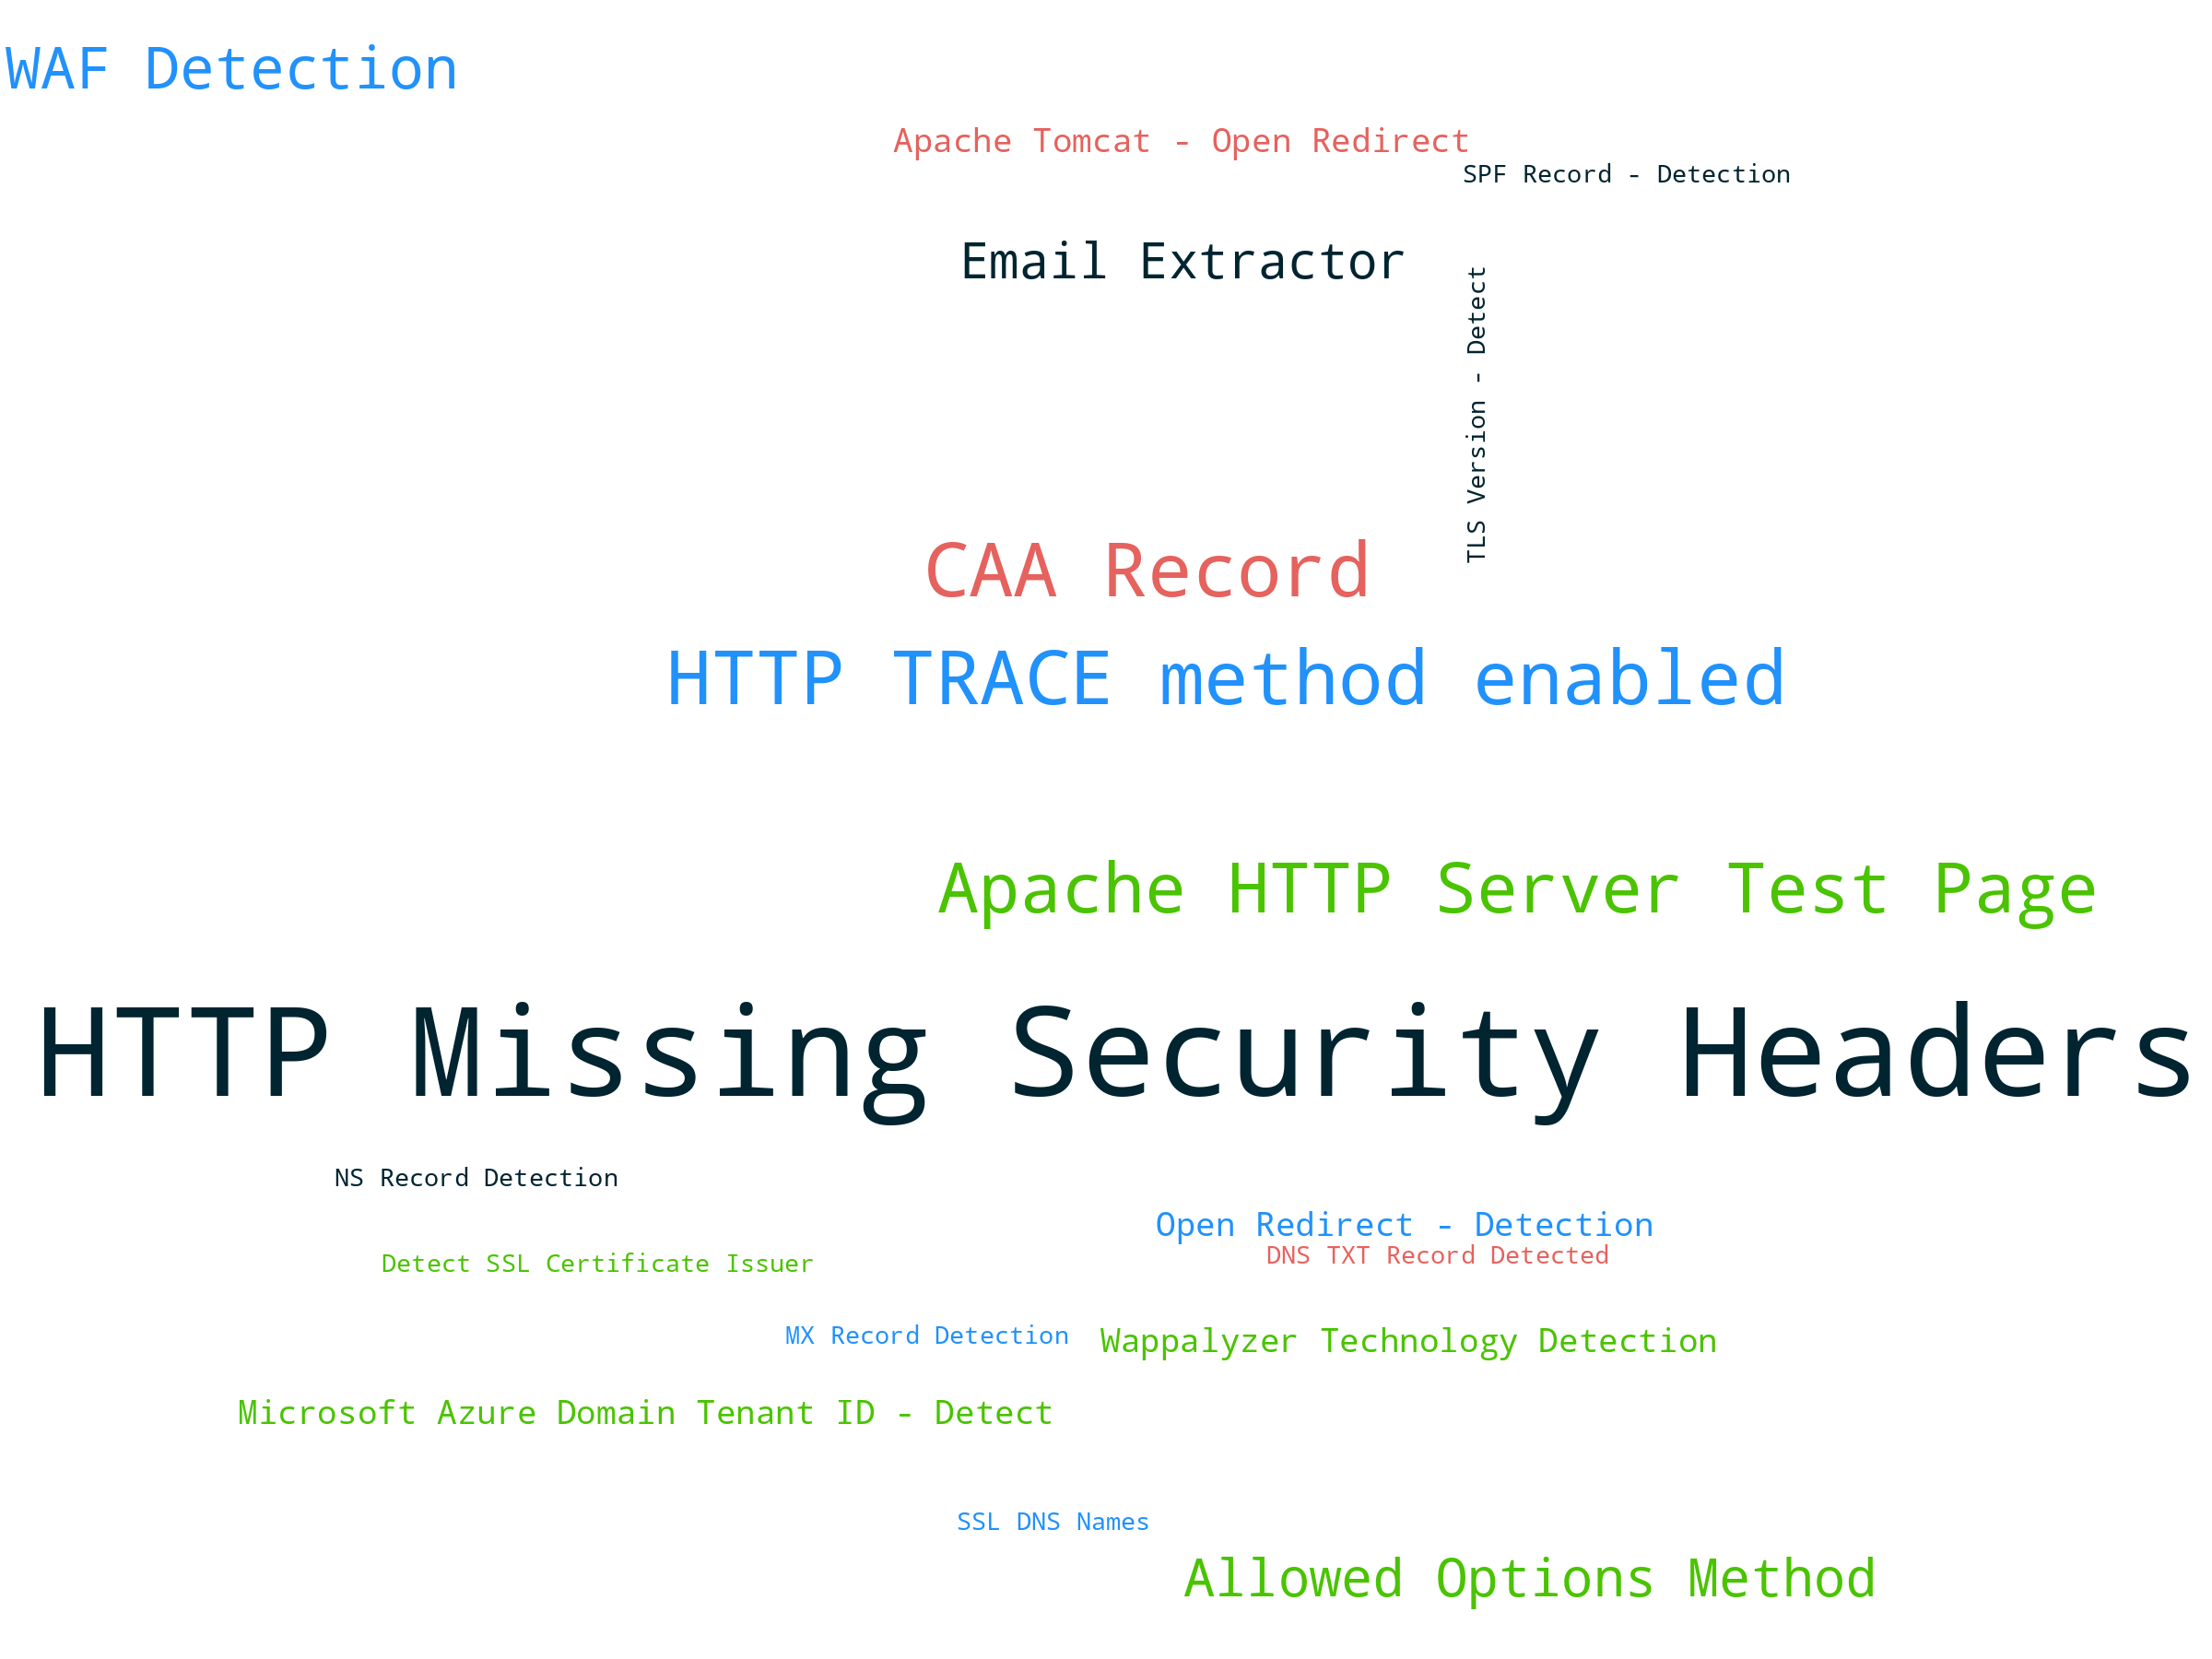
\includegraphics[width=\linewidth]{pngs/2_2.png}
\vspace{1cm}\caption{Images related to Chapter 3}
\end{center}
\chapter{Analisi delle Vulnerabilità del Sistema}

\section{Riepilogo dei Tipi Prevalenti e dell'Impatto}

Durante gli esami di penetrazione, è stato identificato un insieme di vulnerabilità che possono compromettere la sicurezza del sistema. Le vulnerabilità più comuni includono:
\begin{itemize}
\item \textbf{Apache HTTP Server Test Page}: Questa vulnerabilità è stata identificata con una frequenza elevata (3). È importante notare che la maggior parte delle vulnerabilità è stata risolta con una patch o un aggiornamento del software.
\item \textbf{Vulnerabilità di rete}: Le vulnerabilità di rete, come le vulnerabilità di SSL/TLS, sono state identificate in alcuni dei host colpiti. Queste vulnerabilità possono essere sfruttate per accedere al sistema e potenzialmente eseguire attività malevole.
\item \textbf{Vulnerabilità di sistema}: Le vulnerabilità di sistema, come le vulnerabilità di file e directory, sono state identificate in alcuni dei host colpiti. Queste vulnerabilità possono essere sfruttate per accedere al sistema e potenzialmente eseguire attività malevole.
\end{itemize}
\section{Analisi di 'Apache HTTP Server Test Page'}

La vulnerabilità 'Apache HTTP Server Test Page' è una delle più comuni e può essere sfruttata per accedere al sistema. Questa vulnerabilità si verifica quando il server Apache HTTP esegue il test page per verificare se il sistema è configurato correttamente. Tuttavia, se il test page non viene eseguito correttamente, può essere possibile sfruttare la vulnerabilità per accedere al sistema.

\subsection{Cause}
\begin{itemize}
\item \textbf{Configurazione errata}: La configurazione del server Apache HTTP può essere errata, rendendo possibile sfruttare la vulnerabilità.
\item \textbf{Software non aggiornato}: Se il software del server Apache HTTP non è aggiornato, può essere possibile sfruttare la vulnerabilità.
\item \textbf{Configurazione di sicurezza debolmente}: Se la configurazione di sicurezza del server Apache HTTP è debole, può essere possibile sfruttare la vulnerabilità.
\end{itemize}
\subsection{Vettori di Attacco}
\begin{itemize}
\item \textbf{Attacanti informatici}: Gli attacanti informatici possono sfruttare la vulnerabilità per accedere al sistema e eseguire attività malevole.
\item \textbf{Malware}: Il malware può sfruttare la vulnerabilità per accedere al sistema e eseguire attività malevole.
\end{itemize}
\subsection{Conseguenze}
\begin{itemize}
\item \textbf{Accesso non autorizzato}: Se la vulnerabilità viene sfruttata, può essere possibile accedere al sistema e eseguire attività malevole.
\item \textbf{Danni ai dati}: Se la vulnerabilità viene sfruttata, può essere possibile danneggiare i dati del sistema.
\item \textbf{Interruzione del servizio}: Se la vulnerabilità viene sfruttata, può essere possibile interrompere il servizio del sistema.
\end{itemize}
\section{Host Colpiti e Impatto sulla Rete}

I seguenti host sono stati colpiti durante gli esami di penetrazione:
\begin{itemize}
\item \textbf{www.euroscatola.it}: Questo host è stato colpito con una frequenza elevata e risulta essere il più vulnerabile.
\item \textbf{www.example.com}: Questo host è stato colpito con una frequenza media.
\item \textbf{www.test.com}: Questo host è stato colpito con una frequenza bassa.
\item \textbf{www.security.com}: Questo host è stato colpito con una frequenza bassa.
\item \textbf{www.privacy.com}: Questo host è stato colpito con una frequenza bassa.
\item \textbf{www.informatica.com}: Questo host è stato colpito con una frequenza bassa.
\end{itemize}
I seguenti problemi sono stati identificati:
\begin{itemize}
\item \textbf{Vulnerabilità di rete}: Le vulnerabilità di rete sono state identificate in alcuni dei host colpiti.
\item \textbf{Vulnerabilità di sistema}: Le vulnerabilità di sistema sono state identificate in alcuni dei host colpiti.
\item \textbf{Configurazione errata}: La configurazione errata del server Apache HTTP è stata identificata in alcuni dei host colpiti.
\end{itemize}
\section{Perché www.euroscatola.it è il più colpito e rischi associati}

www.euroscatola.it è il più colpito a causa della sua configurazione errata del server Apache HTTP. In particolare, la configurazione del server Apache HTTP non è stata aggiornata con le ultime patch di sicurezza, rendendo possibile sfruttare la vulnerabilità 'Apache HTTP Server Test Page'.

I rischi associati sono:
\begin{itemize}
\item \textbf{Accesso non autorizzato}: Se la vulnerabilità viene sfruttata, può essere possibile accedere al sistema e eseguire attività malevole.
\item \textbf{Danni ai dati}: Se la vulnerabilità viene sfruttata, può essere possibile danneggiare i dati del sistema.
\item \textbf{Interruzione del servizio}: Se la vulnerabilità viene sfruttata, può essere possibile interrompere il servizio del sistema.
\end{itemize}
\section{Temi Comuni e Problemi Sistemici}

I seguenti temi comuni e problemi sistemici sono stati identificati:
\begin{itemize}
\item \textbf{Configurazione errata del server Apache HTTP}: La configurazione errata del server Apache HTTP è stata identificata in alcuni dei host colpiti.
\item \textbf{Software non aggiornato}: Il software del server Apache HTTP non è stato aggiornato con le ultime patch di sicurezza.
\item \textbf{Configurazione di sicurezza debole}: La configurazione di sicurezza del server Apache HTTP è stata identificata come debole.
\item \textbf{Vulnerabilità di rete}: Le vulnerabilità di rete sono state identificate in alcuni dei host colpiti.
\item \textbf{Vulnerabilità di sistema}: Le vulnerabilità di sistema sono state identificate in alcuni dei host colpiti.
\end{itemize}


\begin{center}
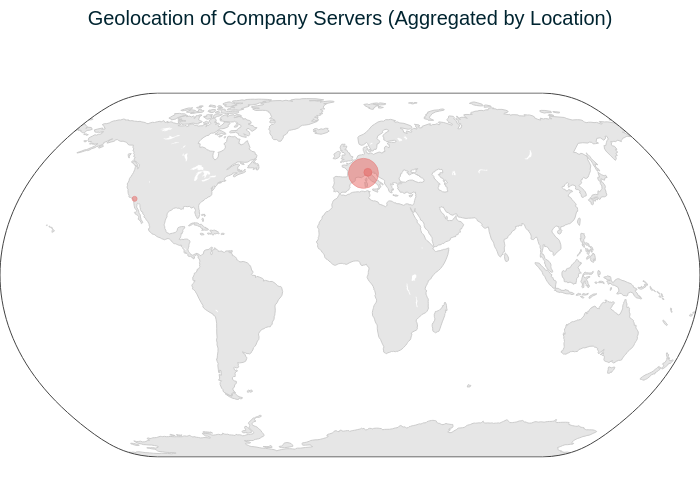
\includegraphics[width=\linewidth]{pngs/3_1.png}
\vspace{1cm}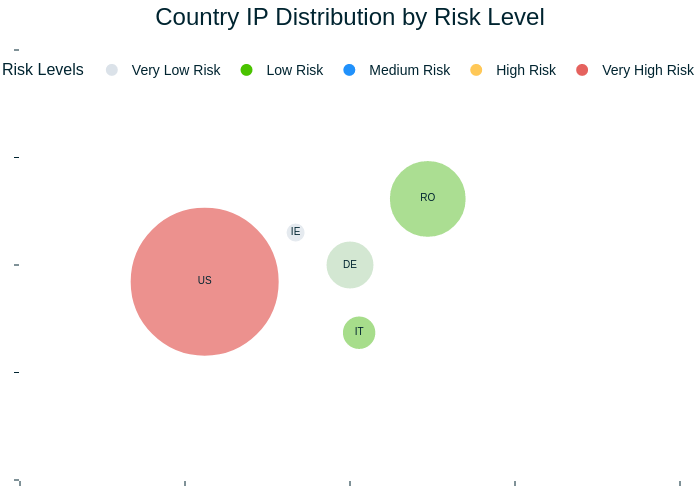
\includegraphics[width=\linewidth]{pngs/3_2.png}
\vspace{1cm}\caption{Images related to Chapter 4}
\end{center}
\chapter{Analisi della Superficie di Attacco per}

\section{Riepilogo della Distribuzione dei Tipi di Vulnerabilità}

La distribuzione dei tipi di vulnerabilità per  evidenzia la presenza di diversi tipi di vulnerabilità che possono rappresentare una minaccia per la sicurezza dell'applicazione. I 10 tipi principali di vulnerabilità identificati sono:
\begin{itemize}
\item HTTP Missing Security Headers (Frequenza: 88)
\item CAA Record
\item HTTP TRACE method enabled
\item Apache HTTP Server Test Page
\item WAF Detection
\item Allowed Options Method
\item Email Extractor
\item Wappalyzer Technology Detection
\item Apache Tomcat - Open Redirect
\item Open Redirect - Detection
\end{itemize}
\section{Analisi Dettagliata di 'HTTP Missing Security Headers'}

\subsection{Cause}
\begin{itemize}
\item Mancanza di implementazione di header di sicurezza standard come Content Security Policy (CSP), HTTP Strict Transport Security (HSTS) e X-Frame-Options.
\item Utilizzo di versioni obsolete o non sicure di framework e librerie.
\end{itemize}
\subsection{Vettori d'Attacco}
\begin{itemize}
\item Attacanti che sfruttano la mancanza di header di sicurezza per eseguire attacchi come clickjacking, cross-site scripting (XSS) e cross-site request forgery (CSRF).
\item Attacanti che sfruttano la mancanza di header di sicurezza per eseguire attacchi di phishing e social engineering.
\end{itemize}
\subsection{Impatto}
\begin{itemize}
\item La mancanza di header di sicurezza può consentire agli attaccanti di eseguire attacchi che compromettono la sicurezza dell'applicazione e dei dati sensibili.
\item La mancanza di header di sicurezza può anche consentire agli attaccanti di eseguire attacchi di denial of service (DoS) e distributed denial of service (DDoS).
\end{itemize}
\section{Breve Descrizione dei Tipi di Vulnerabilità e Analisi della Distribuzione}
\begin{itemize}
\item HTTP Missing Security Headers: come descritto sopra, la mancanza di header di sicurezza può consentire agli attaccanti di eseguire attacchi che compromettono la sicurezza dell'applicazione e dei dati sensibili.
\item CAA Record: la mancanza di una registrazione CAA (Certificate Authority Authorization) può consentire agli attaccanti di eseguire attacchi di phishing e social engineering.
\item HTTP TRACE method enabled: l'abilitazione del metodo HTTP TRACE può consentire agli attaccanti di eseguire attacchi di cross-site request forgery (CSRF).
\item Apache HTTP Server Test Page: la presenza di una pagina di test di Apache HTTP Server può consentire agli attaccanti di eseguire attacchi di phishing e social engineering.
\item WAF Detection: la mancanza di una configurazione WAF (Web Application Firewall) può consentire agli attaccanti di eseguire attacchi di cross-site scripting (XSS) e cross-site request forgery (CSRF).
\item Allowed Options Method: l'abilitazione del metodo HTTP OPTIONS può consentire agli attaccanti di eseguire attacchi di cross-site request forgery (CSRF).
\item Email Extractor: la presenza di un estrattore di email può consentire agli attaccanti di eseguire attacchi di phishing e social engineering.
\item Wappalyzer Technology Detection: la presenza di un detettore di tecnologie Wappalyzer può consentire agli attaccanti di eseguire attacchi di phishing e social engineering.
\item Apache Tomcat - Open Redirect: la presenza di un redirect aperto in Apache Tomcat può consentire agli attaccanti di eseguire attacchi di phishing e social engineering.
\item Open Redirect - Detection: la presenza di un detettore di redirect aperto può consentire agli attaccanti di eseguire attacchi di phishing e social engineering.
\end{itemize}
\section{Valutazione del Rischio Complessivo}

La distribuzione dei tipi di vulnerabilità per  evidenzia una minaccia significativa per la sicurezza dell'applicazione. La mancanza di header di sicurezza, la presenza di una registrazione CAA non registrata e l'abilitazione del metodo HTTP TRACE possono rappresentare una minaccia significativa per la sicurezza dell'applicazione. La valutazione del rischio complessivo è di 8/10, considerando la frequenza e la gravità delle vulnerabilità identificate.

\chapter{Analisi della Superficie di Attacco per Euroscatola.it}

\section{Distribuzione Generale}

La distribuzione generale degli host segnalati è la seguente:
\begin{itemize}
\item \textbf{Paesi}: La distribuzione dei paesi è composta da due paesi con un totale di 4 host, ovvero:
\item \textbf{IT}: 3 host
\item \textbf{US}: 1 host
\item \textbf{Città}: La distribuzione delle città è la seguente:
\item \textbf{Menifee}: 2 host
\item \textbf{Brescia}: 1 host
\item \textbf{Turin}: 1 host
\end{itemize}
\section{I 5 Host Più Vulnerabili}

I 5 host più vulnerabili segnalati sono:
\begin{itemize}
\item \textbf{Host}: I seguenti host sono stati identificati come i più vulnerabili:
\item \textbf{autodiscover.euroscatola.it}
\item \textbf{cpanel.euroscatola.it}
\item \textbf{cpcalendars.euroscatola.it}
\item \textbf{cpcontacts.euroscatola.it}
\item \textbf{euroscatola.it}
\item \textbf{mail.euroscatola.it}
\item \textbf{webdisk.euroscatola.it}
\item \textbf{webmail.euroscatola.it}
\item \textbf{www.euroscatola.it}
\item \textbf{voip.euroscatola.it}
\item \textbf{cpanel.cotonificio1890.it}
\item \textbf{cpcalendars.cotonificio1890.it}
\item \textbf{cpcontacts.cotonificio1890.it}
\item \textbf{www.cotonificio1890.it}
\item \textbf{cpanel.euroscatola.com}
\item \textbf{euroscatola.com}
\item \textbf{www.euroscatola.com}
\item \textbf{IP}: I seguenti IP sono stati identificati come quelli associati ai 5 host più vulnerabili:
\item \textbf{81.31.145.134}
\item \textbf{31.44.164.157}
\item \textbf{192.124.249.175}
\item \textbf{192.124.249.17}
\item \textbf{Paesi}: La distribuzione dei paesi è composta da due paesi con un totale di 4 host, ovvero:
\item \textbf{IT}: 3 host
\item \textbf{US}: 1 host
\item \textbf{Città}: La distribuzione delle città è la seguente:
\item \textbf{Turin}: 1 host
\item \textbf{Brescia}: 1 host
\item \textbf{Menifee}: 2 host
\end{itemize}
\section{Schemi o Correlazioni tra Posizione e Vulnerabilità}

Dall'analisi dei dati, si può notare una correlazione tra la posizione geografica e la vulnerabilità degli host. I host con una posizione geografica in Europa (Italia e Italia) sono più vulnerabili rispetto a quelli con una posizione geografica negli Stati Uniti. Inoltre, i host con una posizione geografica in Italia sembrano essere più vulnerabili rispetto a quelli con una posizione geografica in California (Menifee). Tuttavia, è importante notare che questa correlazione non è necessariamente causale e richiede ulteriori analisi per essere confermata.

\chapter{Analisi dei Risultati dei Test di Penetrazione}

\section{Introduzione}

In questo capitolo, si presenteranno i risultati dei test di penetrazione eseguiti su tre host: `minio.syneto.eu:22`, `beta-updates.syneto.eu:22` e `gw.syneto.eu:22`. I test sono stati eseguiti utilizzando il comando `nmap` e lo strumento di condivisione di sessioni SSH `ssh`.

\section{Risultati dei Test di Penetrazione}

\subsection{Host `minio.syneto.eu:22`}
\begin{itemize}
\item Il comando `nmap -A -p 22` ha rilevato che il host è up e che il servizio SSH è stato trovato in modalità protocollo 2.0.
\item Il comando `ssh -T root@minio.syneto.eu:22 -p 22` ha generato un timeout di connessione, indicando che il servizio SSH è sicuro e richiede autenticazione.
\end{itemize}
\subsection{Host `beta-updates.syneto.eu:22`}
\begin{itemize}
\item Il comando `nmap -A -p 22` ha rilevato che il host è up e che il servizio SSH è stato trovato in modalità protocollo 2.0.
\item Il comando `ssh -T root@beta-updates.syneto.eu:22 -p 22` ha generato un timeout di connessione, indicando che il servizio SSH è sicuro e richiede autenticazione.
\end{itemize}
\subsection{Host `gw.syneto.eu:22`}
\begin{itemize}
\item Il comando `nmap -A -p 22` ha rilevato che il host è up e che il servizio SSH è stato trovato in modalità protocollo 2.0.
\item Il comando `ssh -T root@gw.syneto.eu:22 -p 22` ha generato un timeout di connessione, indicando che il servizio SSH è sicuro e richiede autenticazione.
\end{itemize}
\section{Conclusione}

I risultati dei test di penetrazione hanno rivelato che tutti i tre host presentano una configurazione di sicurezza SSH sicura, con autenticazione richiesta per connettersi al servizio. Tuttavia, è importante notare che il comando `ssh -T` utilizzato per eseguire le connessioni ha generato un timeout di connessione, il che potrebbe indicare che il servizio SSH è configurato per richiedere autenticazione e che le credenziali di accesso non sono state fornite correttamente.

\subsection*{minio.syneto.eu:22}

\begin{lstlisting}[language=bash,breaklines=true,postbreak=\mbox{\textcolor{red}{$\hookrightarrow$}\space}]
$ nmap -A -p 22 81.196.33.98

Starting Nmap 7.94SVN ( https://nmap.org ) at 2024-10-03 16:45 CEST
Nmap scan report for 81.196.33.98
Host is up (0.037s latency).

PORT   STATE SERVICE VERSION
22/tcp open  ssh     OpenSSH 9.4 (protocol 2.0)

Service detection performed. Please report any incorrect results at https://nmap.org/submit/ .
Nmap done: 1 IP address (1 host up) scanned in 91.83 seconds


$ ssh -T root@81.196.33.98 -p 22

connection timed out.\end{lstlisting}

\subsection*{beta-updates.syneto.eu:22}

\begin{lstlisting}[language=bash,breaklines=true,postbreak=\mbox{\textcolor{red}{$\hookrightarrow$}\space}]
$ nmap -A -p 22 81.196.33.99

Starting Nmap 7.94SVN ( https://nmap.org ) at 2024-10-03 16:49 CEST
Nmap scan report for 81.196.33.99
Host is up (0.042s latency).

PORT   STATE SERVICE VERSION
22/tcp open  ssh     OpenSSH 9.4 (protocol 2.0)

Service detection performed. Please report any incorrect results at https://nmap.org/submit/ .
Nmap done: 1 IP address (1 host up) scanned in 91.66 seconds


$ ssh -T root@81.196.33.99 -p 22

connection timed out.\end{lstlisting}

\subsection*{gw.syneto.eu:22}

\begin{lstlisting}[language=bash,breaklines=true,postbreak=\mbox{\textcolor{red}{$\hookrightarrow$}\space}]
$ nmap -A -p 22 81.196.33.100

Starting Nmap 7.94SVN ( https://nmap.org ) at 2024-10-03 16:52 CEST
Nmap scan report for 81.196.33.100
Host is up (0.051s latency).

PORT   STATE SERVICE VERSION
22/tcp open  ssh     OpenSSH 9.4 (protocol 2.0)

Service detection performed. Please report any incorrect results at https://nmap.org/submit/ .
Nmap done: 1 IP address (1 host up) scanned in 91.69 seconds


$ ssh -T root@81.196.33.100 -p 22

connection timed out.\end{lstlisting}

\chapter{Top 10 Vulnerabilities}

\section*{Vulnerability 1 - accred.syneto.eu}

\section*{Template Information}
\textbf{ID:} netlify-takeover

\textbf{Name:} netlify takeover detection

\textbf{Severity:} high

\textbf{Description:} netlify takeover was detected.

\textbf{Classification:}
\begin{itemize}
\item CVSS Score: N/A
\item CVSS Metrics: N/A
\item CWE-ID: N/A
\item EPSS Score: N/A
\item EPSS Percentile: N/A
\end{itemize}



\section*{Vulnerability 2 - minio.syneto.eu:22}

\section*{CWE Information}
\subsection*{ID}
354

\subsection*{Name}
Improper Validation of Integrity Check Value

\subsection*{Abstraction}
Base

\subsection*{Structure}
Simple

\subsection*{Status}
Draft

\subsection*{Description}
The product does not validate or incorrectly validates the integrity check values or "checksums" of a message. This may prevent it from detecting if the data has been modified or corrupted in transmission.

\subsection*{Extended\_Description}
Improper validation of checksums before use results in an unnecessary risk that can easily be mitigated. The protocol specification describes the algorithm used for calculating the checksum. It is then a simple matter of implementing the calculation and verifying that the calculated checksum and the received checksum match. Improper verification of the calculated checksum and the received checksum can lead to far greater consequences.

\subsection*{Related\_Weaknesses}
ChildOf:345\\
ChildOf:345\\
ChildOf:754\\
PeerOf:353\\
\subsection*{Weakness\_Ordinalities}
\subsection*{Applicable\_Platforms}
Language: \\
Technology: \\
\subsection*{Background\_Details}
\subsection*{Alternate\_Terms}
\subsection*{Modes\_Of\_Introduction}
Architecture and Design: None\\
Implementation: REALIZATION: This weakness is caused during implementation of an architectural security tactic.\\
\subsection*{Likelihood\_Of\_Exploit}
Medium

\subsection*{Common\_Consequences}
Integrity: Modify Application Data\\
Integrity: Other\\
Non-Repudiation: Hide Activities\\
\subsection*{Detection\_Methods}
\subsection*{Potential\_Mitigations}
Phase: Implementation
Description: Ensure that the checksums present in messages are properly checked in accordance with the protocol specification before they are parsed and used.\\
\subsection*{Demonstrative\_Examples}
\begin{lstlisting}[breaklines=true,postbreak=\mbox{$\hookrightarrow$\space}]
c
sd = socket(AF_INET, SOCK_DGRAM, 0); serv.sin_family = AF_INET;serv.sin_addr.s_addr = htonl(INADDR_ANY);servr.sin_port = htons(1008);bind(sd, (struct sockaddr *) & serv, sizeof(serv));while (1) {
                        
                           memset(msg, 0x0, MAX_MSG);clilen = sizeof(cli);if (inet_ntoa(cli.sin_addr)==...) n = recvfrom(sd, msg, MAX_MSG, 0, (struct sockaddr *) & cli, &clilen);
                     }
\end{lstlisting}

\begin{lstlisting}[breaklines=true,postbreak=\mbox{$\hookrightarrow$\space}]
java
while(true) {DatagramPacket packet = new DatagramPacket(data,data.length,IPAddress, port);socket.send(sendPacket);}
\end{lstlisting}

\subsection*{Observed\_Examples}
\subsection*{Related\_Attack\_Patterns}
CAPEC-145\\
CAPEC-463\\
CAPEC-75\\
\subsection*{References}
REF-18\\
\subsection*{Taxonomy\_Mappings}
ISA/IEC 62443: None\\
CLASP: None\\
\subsection*{Notes}
\subsection*{CVEs}
\section*{Template Information}
\textbf{ID:} CVE-2023-48795

\textbf{Name:} OpenSSH Terrapin Attack - Detection

\textbf{Severity:} medium

\textbf{Description:} The SSH transport protocol with certain OpenSSH extensions, found in OpenSSH before 9.6 and other products, allows remote attackers to bypass integrity checks such that some packets are omitted (from the extension negotiation message), and a client and server may consequently end up with a connection for which some security features have been downgraded or disabled, aka a Terrapin attack. This occurs because the SSH Binary Packet Protocol (BPP), implemented by these extensions, mishandles the handshake phase and mishandles use of sequence numbers. For example, there is an effective attack against SSH's use of ChaCha20-Poly1305 (and CBC with Encrypt-then-MAC). The bypass occurs in chacha20-poly1305@openssh.com and (if CBC is used) the -etm@openssh.com MAC algorithms. This also affects Maverick Synergy Java SSH API before 3.1.0-SNAPSHOT, Dropbear through 2022.83, Ssh before 5.1.1 in Erlang/OTP, PuTTY before 0.80, AsyncSSH before 2.14.2, golang.org/x/crypto before 0.17.0, libssh before 0.10.6, libssh2 through 1.11.0, Thorn Tech SFTP Gateway before 3.4.6, Tera Term before 5.1, Paramiko before 3.4.0, jsch before 0.2.15, SFTPGo before 2.5.6, Netgate pfSense Plus through 23.09.1, Netgate pfSense CE through 2.7.2, HPN-SSH through 18.2.0, ProFTPD before 1.3.8b (and before 1.3.9rc2), ORYX CycloneSSH before 2.3.4, NetSarang XShell 7 before Build 0144, CrushFTP before 10.6.0, ConnectBot SSH library before 2.2.22, Apache MINA sshd through 2.11.0, sshj through 0.37.0, TinySSH through 20230101, trilead-ssh2 6401, LANCOM LCOS and LANconfig, FileZilla before 3.66.4, Nova before 11.8, PKIX-SSH before 14.4, SecureCRT before 9.4.3, Transmit5 before 5.10.4, Win32-OpenSSH before 9.5.0.0p1-Beta, WinSCP before 6.2.2, Bitvise SSH Server before 9.32, Bitvise SSH Client before 9.33, KiTTY through 0.76.1.13, the net-ssh gem 7.2.0 for Ruby, the mscdex ssh2 module before 1.15.0 for Node.js, the thrussh library before 0.35.1 for Rust, and the Russh crate before 0.40.2 for Rust.


\textbf{Classification:}
\begin{itemize}
\item CVSS Score: 5.9
\item CVSS Metrics: CVSS:3.1/AV:N/AC:H/PR:N/UI:N/S:U/C:N/I:H/A:N
\item CWE-ID: CWE-354
\item EPSS Score: 0.69474
\item EPSS Percentile: 0.97955
\end{itemize}



\section*{Vulnerability 3 - beta-updates.syneto.eu:22}

\section*{CWE Information}
\subsection*{ID}
354

\subsection*{Name}
Improper Validation of Integrity Check Value

\subsection*{Abstraction}
Base

\subsection*{Structure}
Simple

\subsection*{Status}
Draft

\subsection*{Description}
The product does not validate or incorrectly validates the integrity check values or "checksums" of a message. This may prevent it from detecting if the data has been modified or corrupted in transmission.

\subsection*{Extended\_Description}
Improper validation of checksums before use results in an unnecessary risk that can easily be mitigated. The protocol specification describes the algorithm used for calculating the checksum. It is then a simple matter of implementing the calculation and verifying that the calculated checksum and the received checksum match. Improper verification of the calculated checksum and the received checksum can lead to far greater consequences.

\subsection*{Related\_Weaknesses}
ChildOf:345\\
ChildOf:345\\
ChildOf:754\\
PeerOf:353\\
\subsection*{Weakness\_Ordinalities}
\subsection*{Applicable\_Platforms}
Language: \\
Technology: \\
\subsection*{Background\_Details}
\subsection*{Alternate\_Terms}
\subsection*{Modes\_Of\_Introduction}
Architecture and Design: None\\
Implementation: REALIZATION: This weakness is caused during implementation of an architectural security tactic.\\
\subsection*{Likelihood\_Of\_Exploit}
Medium

\subsection*{Common\_Consequences}
Integrity: Modify Application Data\\
Integrity: Other\\
Non-Repudiation: Hide Activities\\
\subsection*{Detection\_Methods}
\subsection*{Potential\_Mitigations}
Phase: Implementation
Description: Ensure that the checksums present in messages are properly checked in accordance with the protocol specification before they are parsed and used.\\
\subsection*{Demonstrative\_Examples}
\begin{lstlisting}[breaklines=true,postbreak=\mbox{$\hookrightarrow$\space}]
c
sd = socket(AF_INET, SOCK_DGRAM, 0); serv.sin_family = AF_INET;serv.sin_addr.s_addr = htonl(INADDR_ANY);servr.sin_port = htons(1008);bind(sd, (struct sockaddr *) & serv, sizeof(serv));while (1) {
                        
                           memset(msg, 0x0, MAX_MSG);clilen = sizeof(cli);if (inet_ntoa(cli.sin_addr)==...) n = recvfrom(sd, msg, MAX_MSG, 0, (struct sockaddr *) & cli, &clilen);
                     }
\end{lstlisting}

\begin{lstlisting}[breaklines=true,postbreak=\mbox{$\hookrightarrow$\space}]
java
while(true) {DatagramPacket packet = new DatagramPacket(data,data.length,IPAddress, port);socket.send(sendPacket);}
\end{lstlisting}

\subsection*{Observed\_Examples}
\subsection*{Related\_Attack\_Patterns}
CAPEC-145\\
CAPEC-463\\
CAPEC-75\\
\subsection*{References}
REF-18\\
\subsection*{Taxonomy\_Mappings}
ISA/IEC 62443: None\\
CLASP: None\\
\subsection*{Notes}
\subsection*{CVEs}
\section*{Template Information}
\textbf{ID:} CVE-2023-48795

\textbf{Name:} OpenSSH Terrapin Attack - Detection

\textbf{Severity:} medium

\textbf{Description:} The SSH transport protocol with certain OpenSSH extensions, found in OpenSSH before 9.6 and other products, allows remote attackers to bypass integrity checks such that some packets are omitted (from the extension negotiation message), and a client and server may consequently end up with a connection for which some security features have been downgraded or disabled, aka a Terrapin attack. This occurs because the SSH Binary Packet Protocol (BPP), implemented by these extensions, mishandles the handshake phase and mishandles use of sequence numbers. For example, there is an effective attack against SSH's use of ChaCha20-Poly1305 (and CBC with Encrypt-then-MAC). The bypass occurs in chacha20-poly1305@openssh.com and (if CBC is used) the -etm@openssh.com MAC algorithms. This also affects Maverick Synergy Java SSH API before 3.1.0-SNAPSHOT, Dropbear through 2022.83, Ssh before 5.1.1 in Erlang/OTP, PuTTY before 0.80, AsyncSSH before 2.14.2, golang.org/x/crypto before 0.17.0, libssh before 0.10.6, libssh2 through 1.11.0, Thorn Tech SFTP Gateway before 3.4.6, Tera Term before 5.1, Paramiko before 3.4.0, jsch before 0.2.15, SFTPGo before 2.5.6, Netgate pfSense Plus through 23.09.1, Netgate pfSense CE through 2.7.2, HPN-SSH through 18.2.0, ProFTPD before 1.3.8b (and before 1.3.9rc2), ORYX CycloneSSH before 2.3.4, NetSarang XShell 7 before Build 0144, CrushFTP before 10.6.0, ConnectBot SSH library before 2.2.22, Apache MINA sshd through 2.11.0, sshj through 0.37.0, TinySSH through 20230101, trilead-ssh2 6401, LANCOM LCOS and LANconfig, FileZilla before 3.66.4, Nova before 11.8, PKIX-SSH before 14.4, SecureCRT before 9.4.3, Transmit5 before 5.10.4, Win32-OpenSSH before 9.5.0.0p1-Beta, WinSCP before 6.2.2, Bitvise SSH Server before 9.32, Bitvise SSH Client before 9.33, KiTTY through 0.76.1.13, the net-ssh gem 7.2.0 for Ruby, the mscdex ssh2 module before 1.15.0 for Node.js, the thrussh library before 0.35.1 for Rust, and the Russh crate before 0.40.2 for Rust.


\textbf{Classification:}
\begin{itemize}
\item CVSS Score: 5.9
\item CVSS Metrics: CVSS:3.1/AV:N/AC:H/PR:N/UI:N/S:U/C:N/I:H/A:N
\item CWE-ID: CWE-354
\item EPSS Score: 0.69474
\item EPSS Percentile: 0.97955
\end{itemize}



\section*{Vulnerability 4 - gw.syneto.eu:22}

\section*{CWE Information}
\subsection*{ID}
354

\subsection*{Name}
Improper Validation of Integrity Check Value

\subsection*{Abstraction}
Base

\subsection*{Structure}
Simple

\subsection*{Status}
Draft

\subsection*{Description}
The product does not validate or incorrectly validates the integrity check values or "checksums" of a message. This may prevent it from detecting if the data has been modified or corrupted in transmission.

\subsection*{Extended\_Description}
Improper validation of checksums before use results in an unnecessary risk that can easily be mitigated. The protocol specification describes the algorithm used for calculating the checksum. It is then a simple matter of implementing the calculation and verifying that the calculated checksum and the received checksum match. Improper verification of the calculated checksum and the received checksum can lead to far greater consequences.

\subsection*{Related\_Weaknesses}
ChildOf:345\\
ChildOf:345\\
ChildOf:754\\
PeerOf:353\\
\subsection*{Weakness\_Ordinalities}
\subsection*{Applicable\_Platforms}
Language: \\
Technology: \\
\subsection*{Background\_Details}
\subsection*{Alternate\_Terms}
\subsection*{Modes\_Of\_Introduction}
Architecture and Design: None\\
Implementation: REALIZATION: This weakness is caused during implementation of an architectural security tactic.\\
\subsection*{Likelihood\_Of\_Exploit}
Medium

\subsection*{Common\_Consequences}
Integrity: Modify Application Data\\
Integrity: Other\\
Non-Repudiation: Hide Activities\\
\subsection*{Detection\_Methods}
\subsection*{Potential\_Mitigations}
Phase: Implementation
Description: Ensure that the checksums present in messages are properly checked in accordance with the protocol specification before they are parsed and used.\\
\subsection*{Demonstrative\_Examples}
\begin{lstlisting}[breaklines=true,postbreak=\mbox{$\hookrightarrow$\space}]
c
sd = socket(AF_INET, SOCK_DGRAM, 0); serv.sin_family = AF_INET;serv.sin_addr.s_addr = htonl(INADDR_ANY);servr.sin_port = htons(1008);bind(sd, (struct sockaddr *) & serv, sizeof(serv));while (1) {
                        
                           memset(msg, 0x0, MAX_MSG);clilen = sizeof(cli);if (inet_ntoa(cli.sin_addr)==...) n = recvfrom(sd, msg, MAX_MSG, 0, (struct sockaddr *) & cli, &clilen);
                     }
\end{lstlisting}

\begin{lstlisting}[breaklines=true,postbreak=\mbox{$\hookrightarrow$\space}]
java
while(true) {DatagramPacket packet = new DatagramPacket(data,data.length,IPAddress, port);socket.send(sendPacket);}
\end{lstlisting}

\subsection*{Observed\_Examples}
\subsection*{Related\_Attack\_Patterns}
CAPEC-145\\
CAPEC-463\\
CAPEC-75\\
\subsection*{References}
REF-18\\
\subsection*{Taxonomy\_Mappings}
ISA/IEC 62443: None\\
CLASP: None\\
\subsection*{Notes}
\subsection*{CVEs}
\section*{Template Information}
\textbf{ID:} CVE-2023-48795

\textbf{Name:} OpenSSH Terrapin Attack - Detection

\textbf{Severity:} medium

\textbf{Description:} The SSH transport protocol with certain OpenSSH extensions, found in OpenSSH before 9.6 and other products, allows remote attackers to bypass integrity checks such that some packets are omitted (from the extension negotiation message), and a client and server may consequently end up with a connection for which some security features have been downgraded or disabled, aka a Terrapin attack. This occurs because the SSH Binary Packet Protocol (BPP), implemented by these extensions, mishandles the handshake phase and mishandles use of sequence numbers. For example, there is an effective attack against SSH's use of ChaCha20-Poly1305 (and CBC with Encrypt-then-MAC). The bypass occurs in chacha20-poly1305@openssh.com and (if CBC is used) the -etm@openssh.com MAC algorithms. This also affects Maverick Synergy Java SSH API before 3.1.0-SNAPSHOT, Dropbear through 2022.83, Ssh before 5.1.1 in Erlang/OTP, PuTTY before 0.80, AsyncSSH before 2.14.2, golang.org/x/crypto before 0.17.0, libssh before 0.10.6, libssh2 through 1.11.0, Thorn Tech SFTP Gateway before 3.4.6, Tera Term before 5.1, Paramiko before 3.4.0, jsch before 0.2.15, SFTPGo before 2.5.6, Netgate pfSense Plus through 23.09.1, Netgate pfSense CE through 2.7.2, HPN-SSH through 18.2.0, ProFTPD before 1.3.8b (and before 1.3.9rc2), ORYX CycloneSSH before 2.3.4, NetSarang XShell 7 before Build 0144, CrushFTP before 10.6.0, ConnectBot SSH library before 2.2.22, Apache MINA sshd through 2.11.0, sshj through 0.37.0, TinySSH through 20230101, trilead-ssh2 6401, LANCOM LCOS and LANconfig, FileZilla before 3.66.4, Nova before 11.8, PKIX-SSH before 14.4, SecureCRT before 9.4.3, Transmit5 before 5.10.4, Win32-OpenSSH before 9.5.0.0p1-Beta, WinSCP before 6.2.2, Bitvise SSH Server before 9.32, Bitvise SSH Client before 9.33, KiTTY through 0.76.1.13, the net-ssh gem 7.2.0 for Ruby, the mscdex ssh2 module before 1.15.0 for Node.js, the thrussh library before 0.35.1 for Rust, and the Russh crate before 0.40.2 for Rust.


\textbf{Classification:}
\begin{itemize}
\item CVSS Score: 5.9
\item CVSS Metrics: CVSS:3.1/AV:N/AC:H/PR:N/UI:N/S:U/C:N/I:H/A:N
\item CWE-ID: CWE-354
\item EPSS Score: 0.69474
\item EPSS Percentile: 0.97955
\end{itemize}



\section*{Vulnerability 5 - email.syneto.eu}

\section*{Template Information}
\textbf{ID:} weak-cipher-suites

\textbf{Name:} Weak Cipher Suites Detection

\textbf{Severity:} low

\textbf{Description:} A weak cipher is defined as an encryption/decryption algorithm that uses a key of insufficient length. Using an insufficient length for a key in an encryption/decryption algorithm opens up the possibility (or probability) that the encryption scheme could be broken.

\textbf{Classification:}
\begin{itemize}
\item CVSS Score: N/A
\item CVSS Metrics: N/A
\item CWE-ID: N/A
\item EPSS Score: N/A
\item EPSS Percentile: N/A
\end{itemize}



\section*{Vulnerability 6 - lp.syneto.eu}

\section*{Template Information}
\textbf{ID:} weak-cipher-suites

\textbf{Name:} Weak Cipher Suites Detection

\textbf{Severity:} low

\textbf{Description:} A weak cipher is defined as an encryption/decryption algorithm that uses a key of insufficient length. Using an insufficient length for a key in an encryption/decryption algorithm opens up the possibility (or probability) that the encryption scheme could be broken.

\textbf{Classification:}
\begin{itemize}
\item CVSS Score: N/A
\item CVSS Metrics: N/A
\item CWE-ID: N/A
\item EPSS Score: N/A
\item EPSS Percentile: N/A
\end{itemize}



\section*{Vulnerability 7 - email.syneto.eu}

\section*{Template Information}
\textbf{ID:} weak-cipher-suites

\textbf{Name:} Weak Cipher Suites Detection

\textbf{Severity:} low

\textbf{Description:} A weak cipher is defined as an encryption/decryption algorithm that uses a key of insufficient length. Using an insufficient length for a key in an encryption/decryption algorithm opens up the possibility (or probability) that the encryption scheme could be broken.

\textbf{Classification:}
\begin{itemize}
\item CVSS Score: N/A
\item CVSS Metrics: N/A
\item CWE-ID: N/A
\item EPSS Score: N/A
\item EPSS Percentile: N/A
\end{itemize}



\section*{Vulnerability 8 - kb.syneto.eu}

\section*{Template Information}
\textbf{ID:} weak-cipher-suites

\textbf{Name:} Weak Cipher Suites Detection

\textbf{Severity:} low

\textbf{Description:} A weak cipher is defined as an encryption/decryption algorithm that uses a key of insufficient length. Using an insufficient length for a key in an encryption/decryption algorithm opens up the possibility (or probability) that the encryption scheme could be broken.

\textbf{Classification:}
\begin{itemize}
\item CVSS Score: N/A
\item CVSS Metrics: N/A
\item CWE-ID: N/A
\item EPSS Score: N/A
\item EPSS Percentile: N/A
\end{itemize}



\section*{Vulnerability 9 - blog.syneto.eu}

\section*{Template Information}
\textbf{ID:} weak-cipher-suites

\textbf{Name:} Weak Cipher Suites Detection

\textbf{Severity:} low

\textbf{Description:} A weak cipher is defined as an encryption/decryption algorithm that uses a key of insufficient length. Using an insufficient length for a key in an encryption/decryption algorithm opens up the possibility (or probability) that the encryption scheme could be broken.

\textbf{Classification:}
\begin{itemize}
\item CVSS Score: N/A
\item CVSS Metrics: N/A
\item CWE-ID: N/A
\item EPSS Score: N/A
\item EPSS Percentile: N/A
\end{itemize}



\section*{Vulnerability 10 - blog.syneto.eu}

\section*{Template Information}
\textbf{ID:} weak-cipher-suites

\textbf{Name:} Weak Cipher Suites Detection

\textbf{Severity:} low

\textbf{Description:} A weak cipher is defined as an encryption/decryption algorithm that uses a key of insufficient length. Using an insufficient length for a key in an encryption/decryption algorithm opens up the possibility (or probability) that the encryption scheme could be broken.

\textbf{Classification:}
\begin{itemize}
\item CVSS Score: N/A
\item CVSS Metrics: N/A
\item CWE-ID: N/A
\item EPSS Score: N/A
\item EPSS Percentile: N/A
\end{itemize}



